

\documentclass{article}
\usepackage[utf8]{inputenc}
\usepackage{hyperref}
\usepackage{listings}
\usepackage{color}
\usepackage{graphicx} % Required for inserting images
\usepackage{amsmath}
\usepackage{markdown}

\definecolor{codegreen}{rgb}{0,0.6,0}
\definecolor{codegray}{rgb}{0.5,0.5,0.5}
\definecolor{codepurple}{rgb}{0.58,0,0.82}
\definecolor{backcolour}{rgb}{0.95,0.95,0.92}

\lstdefinelanguage{Toml}{
    comment = [l]{\#},
    keywords = {true, false},
    morestring = [b]{"}
}

% Thanks to https://chat.openai.com/g/g-eW4YzRIyC-note-converter
\lstdefinestyle{mystyle}{
    backgroundcolor=\color{backcolour},   
    commentstyle=\color{codegreen},
    keywordstyle=\color{magenta},
    numberstyle=\tiny\color{codegray},
    stringstyle=\color{codepurple},
    basicstyle=\ttfamily\footnotesize,
    breakatwhitespace=false,         
    breaklines=true,                 
    captionpos=b,                    
    keepspaces=true,                 
    numbers=left,                    
    numbersep=5pt,                  
    showspaces=false,                
    showstringspaces=false,
    showtabs=false,                  
    tabsize=2
}

\lstset{style=mystyle}

\title{Simulated Annealing - CS 5300}
\author{Austin Hester}
\date{February 2024}

\begin{document}

\maketitle

\section{Problem}

You got a problem?

\subsection{Recommended Schedule}

$$\lambda x : x / 1.2$$

The average traced search path length:

\begin{itemize}
    \item for subpar results $= 99$.
    \item for good results $= 25$.
\end{itemize}

See the $x : x / 1.2$ output graph:

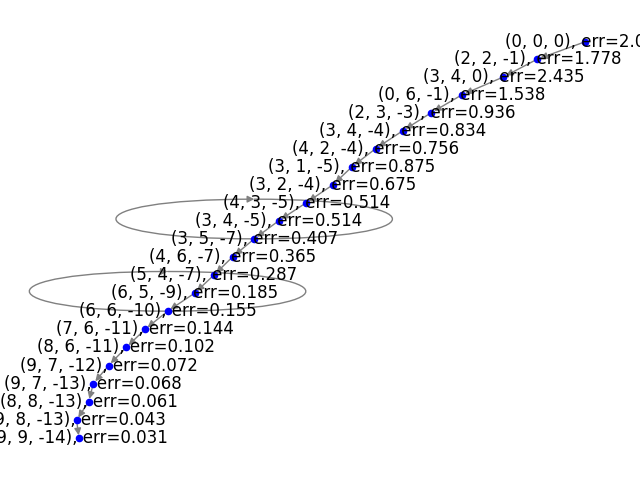
\includegraphics[width=6in]{_static/Figure_3_Temp=1.2_Path=23.png}
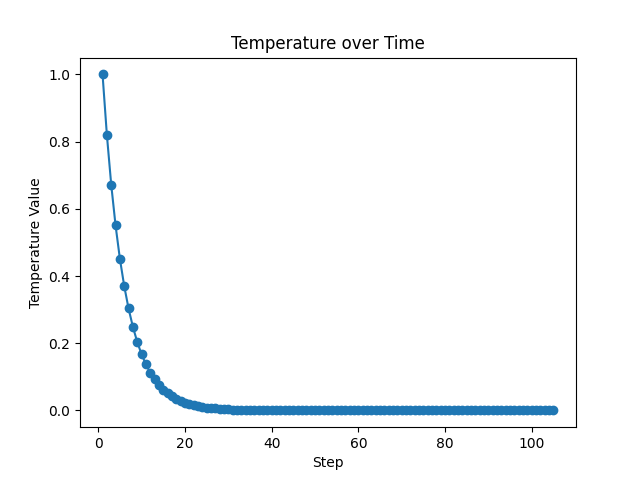
\includegraphics[width=6in]{_static/Figure_6_Temp=1.2_Temp-over-Time.png}
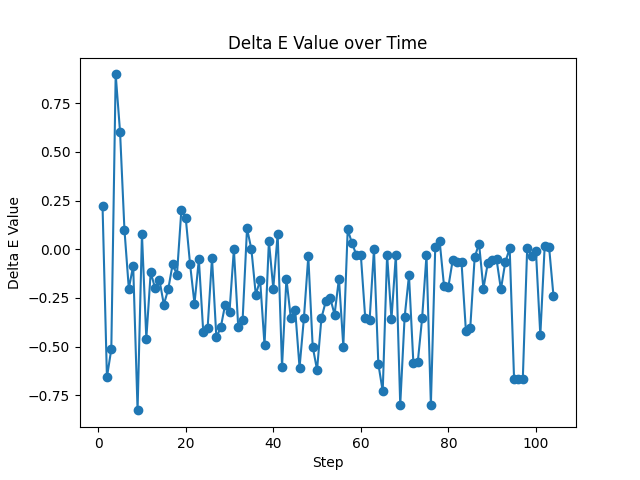
\includegraphics[width=6in]{_static/Figure_9_Temp=1.22_Delta-E-over-Time.png}
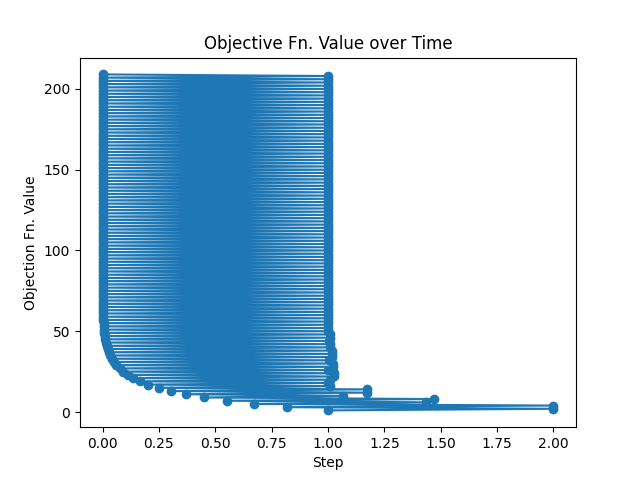
\includegraphics[width=6in]{_static/Figure_10_Temp=1.22_Obj-Fn-over-Time.png}

---

\section{Struggles}

\subsection{Learning Jupyter}

Learning what Jupyter notebook was and getting it to run took a good chunk of 
time out of working on my project. I also had to refactor my entire codebase 
to get it running in Jupyter notebook.

\subsection{Converting Report to LaTeX}

Converting this report to LateX from Markdown as I originally wrote it in
seemed like a waste of time considering that GitHub markdown rendering can 
be very good.

\section{Online Resources}

\begin{enumerate}
    \item GitHub repository: \url{https://github.com/ahester57/ai_workshop}.
    \item Python virtual environments: \url{https://docs.python.org/3/tutorial/venv.html}.
    \item Jupyter Notebook Coach: \url{https://chat.openai.com/g/g-QAzs1b7Si-jupyter-notebook-coach}.
    \item Markdown to LaTex: \url{https://chat.openai.com/g/g-eW4YzRIyC-note-converter}.
\end{enumerate}

\section{Example Output}

\begin{lstlisting}[language=bash, caption=Example Output of Program]
$ aiw
usage: aiw [-h] [-c CONFIG] [-v] [-w WARN] {anneal,svm,convolve} ...

options:
  -h, --help            show this help message and exit
  -c CONFIG, --config CONFIG
                        config file [etc/config.toml]
  -v, --version         print version and exit
  -w WARN, --warn WARN  logger warning level [WARN]

subcommands:
  {anneal,svm,convolve}
\end{lstlisting}

\section{The Code}

\begin{lstlisting}[language=Python, caption=Simulated Annealing Algorithm]
""" Implement the anneal command.

```
function SIMULATED-ANNEALING(problem, schedule) returns a solution State
  current <- problem.INITIAL
  for t = 1 to inf do
      T <- schedule(t)
      if T = 0 then return current
      next <- a randomly selected successor of current
      delta_E <- VALUE(current) - VALUE(next)
      if delta_E > 0 then current <- next
      else current <- next only with probability e^(-delta_E/T)
```

Stuart Russel, Peter Norvig. "Artificial Intelligence: A Modern Approach, 4th Edition" (2021)
"""
import numpy as np

from graphlib import CycleError
from typing import Callable

try:
    # for visual mode. `pip install -e .[visual]
    import matplotlib.pyplot as plt
    import networkx as nx
    DiGraph = nx.DiGraph
except ModuleNotFoundError:
    plt = None
    nx = None
    class DiGraph: pass

from ..core.logger import logger
from ..model.problem import ProblemGraph
from ..model.node import Neuron


def _anneal_step(
        problem:ProblemGraph,
        T:float,
        current:Neuron,
        successor:Neuron,
        G:DiGraph|None=None
    ) -> Neuron:
    """ Execute one step of the simulated annealing function.
    
    :param problem: The problem definition.
    :type problem: ProblemGraph
    :param T: Current temperature.
    :type T: float
    :param current: The current node, searching for a greener pasture.
    :type current: Neuron
    :param successor: One of the neighboring nodes, enticing.
    :type successor: Neuron
    :param G: The network graph, if visual mode enabled.
    :type G: networkx.DiGraph|None
    :return: Either the current or successor node
    :rtype: Neuron
    """
    delta_E = problem.evaluate_node(current) - problem.evaluate_node(successor)
    logger.debug(delta_E)
    if delta_E > 0:
        logger.debug("Taking successor as better option (exploitation)")
        problem.add(successor, current) # Trace the path
        if G is not None:
            G.add_edge(current, successor)
        return successor
    else:
        logger.debug(T)
        probability = np.exp(delta_E / T)
        if np.random.default_rng().uniform() < probability:
            logger.debug("Taking successor with probability %d%s (exploration)", probability*100, '%')
            problem.add(successor, current) # Trace the path
            if G is not None:
                G.add_edge(current, successor)
            return successor
    return current


def _anneal_loop(
        problem:ProblemGraph|None=None,
        schedule:Callable=lambda x : x / 1.2,
        G:DiGraph|None=None
    ) -> Neuron:
    """ Execute the simulated annealing algorithm.
    
    :param problem: The problem definition.
    :type problem: ProblemGraph
    :param schedule: Temperature function
    :type schedule: Callable
    :param G: The network graph, if visual mode enabled.
    :type G: networkx.DiGraph|None
    :return: The winner
    :rtype: Neuron
    """
    logger.debug("executing anneal command")
    assert isinstance(problem, ProblemGraph)
    assert isinstance(schedule, Callable)
    current = problem.initial
    logger.debug("Initial: %s", current)
    T = 1
    for t in range(10000000):
        T = schedule(T)
        if T < 0.000000001: break
        successor = Neuron(
            *current.weights
           + np.random.default_rng()
                .integers(
                    low=-2.-current.error,
                   # widen step size as error increases
                    high=2.+current.error,
                    size=Neuron.DIM_W)
        )
        current = _anneal_step(problem, T, current, successor, G)
    return current


def main(problem:ProblemGraph|None=None, schedule:Callable=lambda x : x / 1.2) -> ProblemGraph:
    """ Entrypoint to the simulated annealing algorithm.
    
    :param problem: The problem definition.
    :type problem: ProblemGraph
    :param schedule: Temperature function
    :type schedule: Callable
    :return: The problem with solution search graph.
    :rtype: ProblemGraph
    """
    logger.debug("executing anneal command")
    assert problem is None or isinstance(problem, ProblemGraph)
    assert schedule is None or isinstance(schedule, Callable)
    if problem is None:
        problem = ProblemGraph(Neuron(0, 0, 0))
    if schedule is None:
        schedule = lambda x : x / 1.2
    for attempt in range(1, 10):
        # Random Restarts 10x or until err < 0.5
        G = None
        if plt is not None and nx is not None:
            G = nx.DiGraph()
        # Run simulated annealing
        winner = _anneal_loop(problem, schedule, G)
        try:
            # Topological sort
            static_order = tuple(problem.static_order())
        except CycleError as cycerr:
            logger.warn(cycerr)
            static_order = 'cycle'
        logger.debug(f"Static Order: {static_order}")
        logger.info("Winner: %s", winner)
        logger.info("Path Length: %s", len(problem.graph.keys()))
        if winner.error < 0.5:
            break
        logger.warn("Winner not good enough, restarting with attempt #%d.", attempt)
        problem = ProblemGraph(Neuron(0, 0, 0))
    if G is not None:
        logger.info("Graph Length: %s", len(G))
        pos = nx.kamada_kawai_layout(G, weight=None)
        nx.draw(G, pos, with_labels=True, node_color='blue', edge_color='grey', node_size=20)
        plt.show()
    return problem


if __name__ == "__main__":
    main()

\end{lstlisting}

\section{Python Package Requirements}

\begin{lstlisting}[language=Toml, caption=Python Project Definition]
[build-system]
requires = ["setuptools>=61.0"]
build-backend = "setuptools.build_meta"

[project]
name = "simulated_annealing"
description = "A simulated annealing process to determine the optimal weight values of an artificial neuron."
authors = [
    { name = "Austin Hester", email = "ahester57@gmail.com" },
]
license = {file = "LICENSE"}
classifiers = [
    "Development Status :: 3 - Alpha",
    "Framework :: Pytest",
    "Intended Audience :: Education",
    "License :: OSI Approved :: MIT License",
    "Programming Language :: Python",
    "Programming Language :: Python :: 3",
    "Programming Language :: Python :: 3.8",
    "Programming Language :: Python :: 3.9",
    "Programming Language :: Python :: 3.10",
    "Programming Language :: Python :: 3.11",
    "Programming Language :: Python :: 3.12",
    "Natural Language :: English",
    "Topic :: Scientific/Engineering :: Artificial Intelligence",
    "Topic :: Education :: Testing"
]
requires-python = ">=3.8"
dependencies = [
    "numpy>=1.26.4,<2",
    "tomli==2.0.1; python_version<'3.11'",
]
dynamic = ["version", "readme"]

[project.urls]
"Homepage" = "https://github.com/ahester57/simulated_annealing"

[project.scripts]
simulated_annealing = "simulated_annealing.cli:main"

[project.optional-dependencies]
deep = [
    "keras>=3.0.5,<4",
    "torch>=2.1.2,<3",
    "torchvision>=0.16.2,<1",
]
dev = [
    "pytest>=7.3.1,<8",
    "sphinx>=6.2.1,<7",
    "sphinx_rtd_theme>=1.2.1,<2",
]
jupyter = [
    "notebook>=7.1.1,<8"
]
visual = [
    "networkx>=3.2.0,<4",
    "matplotlib>=3.8.3,<4",
    "scipy>=1.12.0,<2"
]

[tool.setuptools.dynamic]
version = {attr = "simulated_annealing.__version__"}
readme = {file = ["README.md"], content-type = "text/markdown"}

[tool.setuptools.packages.find]
where = ["src"]
\end{lstlisting}

\section{Further Documentation}

References to additional documentation within the repository.

\end{document}